% ========================================
\section{Numerical experiments}\label{sec:Num-Exp}
% ========================================
%
We present numerical results for both Monte Carlo and multi-fidelity Monte Carlo sampling methods to estimate the expectation $\mathbb{E}(u)$. Following \cite{FaHe:2017}, the computational framework is built upon an ITER reactor geometry featuring twelve magnetic coils, with the \textit{reference currents} $\boldsymbol{I}$ specified as
%
\begin{equation}\label{eq:CentralCurrentValue}
{\renewcommand{\arraycolsep}{2pt}
\begin{array}{llll}
I_1 = -1.4 \times 10^{6} A, \quad & I_2 = -9.5 \times 10^{6} A, \quad & I_3 = -2.0388 \times 10^{7} A, \quad & I_4 = -2.0388 \times 10^{7} A, \\
I_5 = -9 \times 10^{6} A, \quad & I_6 = 3.564 \times 10^{6} A, \quad & I_7 = 5.469 \times 10^{6} A, \quad & I_8 = -2.266 \times 10^{6} A, \\
I_9 = -6.426 \times 10^{6} A, \quad & I_{10} = -4.82 \times 10^{6} A, \quad & I_{11} = -7.504 \times 10^{6} A, \quad & I_{12} = 1.724 \times 10^{7} A. 
\end{array}
}
\end{equation}
%
The profiles for $p$ and $g$ on the right-hand side of \eqref{eq:FreeBoundary} follow the form given in \eqref{eq:source}, using the following \textit{reference parameter} values
%
\begin{equation}\label{eq:CentralParameterValue}
r_0=6.2m,\,\,\beta=0.5978, \,\, \alpha_1 = 2, \,\,  \alpha_2=1.395, \,\, j_0=1.3655 \times 10^6 A/m^2,\,\,  \mu_0=1.2566\times 10^{-6} N/A^2.
\end{equation}
%
The reactor geometry and coil arrangement follow the specifications provided in \cite{Amoskov:2009}. To assess the sensitivity of the solution to \eqref{eq:FreeBoundary} under uncertainty, we introduce perturbations in the coil currents, modeled as uniformly distributed variations of $\tau = 2\%$ around the reference values in \eqref{eq:CentralCurrentValue}. 

% \sout{In the second experiment, uncertainties are introduced in the profile parameters, modeled as uniformly distributed perturbations of $\tau = 1\%$ around the reference values in \eqref{eq:CentralParameterValue}, with the coil currents kept constant.}

To ensure that the discretization error meets the required tolerance and to construct low-fidelity models for MFMC, we generate a family of uniformly refined spatial meshes $\{\mathcal{T}_k\}$ by refining and coarsening the reference ITER geometry. Given that the reactor geometry includes curved boundaries, an accurate numerical approximation requires careful spatial discretization. We thus construct six non-nested spatial discretizations, where the number of spatial grid nodes $\{M_\ell,\}_{0\le \ell \le 5}$ follows the scaling relation
%
\begin{equation}
\label{eq:MeshGrowth}
M_\ell = s M_{\ell-1} \qquad \text{ for } s>1.
\end{equation}
%
The values of $M_\ell$ at each level are reported in Table \ref{Tab:MFMC_parameters_dynamic}. The splitting ratio $\theta$ is chosen to be 0.5 to reflect a balance between the discretization and statistical errors. Tolerances for the normalized mean square error are selected to slightly exceed the discretization error on the finest available mesh $(\ell=5)$, with specific values set as $\epsilon=2\times 10^{-4}, 4\times 10^{-4}, 6\times 10^{-4}, 8\times 10^{-4}, 1\times 10^{-3}, 2\times 10^{-3}, 4\times 10^{-3}, 8\times 10^{-3}$. For each tolerance, the corresponding spatial grid level required to satisfy the discretization error threshold is determined using the relation described in \eqref{eq:SLSGC_MLS_SpatialGridsNo}, yielding levels $L = 5, 4, 4, 4, 4, 3, 3, 2, 2$. The high-fidelity model for each tolerance corresponds to the finite element solution of \eqref{eq:FreeBoundary} at the spatial grid level $L$. 



To perform MFMC sampling, we need to estimate the statistical parameters, including the mean and variance of both high- and low-fidelity models, and correlation coefficients that characterize the correlation between high- and low-fidelity models. Welford's algorithm \cite{Welford:1962} is used to achieve robust and numerically stable updates for these sample statistics. The initialization of the proxies for the mean and variance of the high- and low-fidelity models is set to $m_w^{(1)}=0$, $v_w^{(1)}=0$, $\widehat m_w^{(1)}=0$, and $\widehat v_w^{(1)}=0$, respectively.  For the high-fidelity model  $\widehat u_{h,1}=u_h$, the proxies for the sample mean and variance are updated iteratively as new samples are incorporated through the recurrence relations
%
\[
m_w^{(i)} = m_w^{(i-1)} + \frac{u_h\left(\boldsymbol{\omega}^{(i)}\right)-m_w^{(i-1)}}{i},\qquad v_w^{(i)} = v_w^{(i-1)} + \left\langle u_h\left(\boldsymbol{\omega}^{(i)}\right)-m_w^{(i-1)}, \;\;u_h\left(\boldsymbol{\omega}^{(i)}\right)-m_w^{(i)}\right\rangle,
\]
%
Similarly, for the low-fidelity model $\widehat u_{h,k}$, the proxies are updated using analogous recurrence relations
%
\[
\widehat m_w^{(i)} = \widehat m_w^{(i-1)} + \frac{\widehat u_{h,k}\left(\boldsymbol{\omega}^{(i)}\right) - \widehat m_w^{(i-1)}}{i},\qquad \widehat v_w^{(i)} = \widehat v_w^{(i-1)} + \left\langle \widehat u_{h,k}\left(\boldsymbol{\omega}^{(i)}\right)-\widehat m_w^{(i-1)},\;\; \widehat u_{h,k}\left(\boldsymbol{\omega}^{(i)}\right)-\widehat m_w^{(i)}\right\rangle,
\]
%
The correlation between the high- and low-fidelity models is quantified through the covariance, for which the proxy is initialized as $r_w^{(1)}=0$. The iterative update for the covariance is performed using the relation
%
\[
r_w^{(i)} = r_w^{(i-1)} + \left \langle u_{h}\left(\boldsymbol{\omega}^{(i)}\right)-m_{w}^{(i-1)},\;\;\widehat u_{h,k}\left(\boldsymbol{\omega}^{(i)}\right)-\widehat m_{w}^{(i)}\right\rangle,
\]
%
These iterative updates ensure that the statistical parameters are dynamically adjusted without requiring the storage of all previous samples, thus maintaining computational efficiency. Using these updated proxies, the sample standard deviations of the high- and low-fidelity models are calculated as $\sigma_w^{(i)} = \sqrt{v_w^{(i)}/(i-1)}$ and $\widehat \sigma_w^{(i)} = \sqrt{\widehat v_w^{(i)}/(i-1)}$ respectively. The sample covariance between the high-fidelity model and each low-fidelity model is determined as $\text{Cov}_w^{(i)} = r_w^{(i)}/(i-1)$.

Experiments were performed using MATLAB R2024a on the batch-scheduled HPC/HTC cluster NOTSx, part of the Rice Big Research Data cloud infrastructure. The system consists of 298 dual-socket compute blades housed on HPE s6500, HPE Apollo 2000, and Dell PowerEdge C6400 chassis. All nodes are interconnected via a high-speed network with 10 or 25 Gigabit Ethernet.


% =============================
\subsection{Surrogate construction and parameter estimation (offline) costs}
% =============================
For each high-fidelity model defined on the spatial grid level $L$, we generate a set of candidate low-fidelity surrogates using the sparse grid stochastic collocation approach described in Section \ref{sec:SC}. These surrogates are constructed with sparse grid nodes \eqref{eq:NestedColPts} at level $q=1$ and are defined over a sequence of spatial meshes with grid levels ranging from $0$ to $L-1$, where $L$ corresponds to the spatial grid level of the high-fidelity model. However, not all candidate fidelity models are necessarily used, as their associated parameters must satisfy the conditions outlined in Theorem \ref{thm:Sample_size_est}, which governs the model selection process in MFMC.


Using the high-fidelity model and available low-fidelity surrogates, we next estimate the statistical parameters for MFMC. Accurate parameter estimation often requires a large number of samples, increasing the offline computational cost. To improve efficiency, we introduce a dynamic strategy for parameter estimation that iteratively updates sample statistics using Welford’s method while adaptively increasing sample sizes until the relative change in cost efficiency falls below $10^{-2}$, as outlined in Algorithm \ref{algo:Parameter_Estimation}. This approach incorporates the backtracking strategy from Algorithm \ref{algo:enhanced_mfmc_selection} to enhance efficiency when handling a large number of low-fidelity models. To avoid statistical dependence in parameter estimation, each pairwise correlation coefficient $\rho_{1,k}$ between the high-fidelity model and the $k$-th low-fidelity model is computed using mutually independent sample sets. This independence is crucial to prevent bias in the MFMC estimator. As a result, if there are $K$ low-fidelity models and each $\rho_{1,k}$ requires $N$ independent high-fidelity samples for estimation, the total number of high-fidelity evaluations required is $KN$. Table \ref{Tab:MFMC_parameters_dynamic} presents the estimated standard deviations, correlation coefficients, and cost efficiency for different tolerance levels $\epsilon$, considering all candidate low-fidelity models before selection. To establish a benchmark, Table \ref{Tab:MFMC_parameters} reports results using a fixed sample size of 500 for each high- and low-fidelity pair. A comparison between the two approaches reveals that the correlation coefficients obtained through dynamic sampling and those from the fixed sample size approach are highly consistent, differing by at most two decimal places in most cases. Furthermore, since cost efficiency varies smoothly with correlation coefficients, small deviations in parameter estimates have little impact on the overall performance of the method. This is confirmed by the cost efficiencies computed via \eqref{eq:MFMC_sampling_cost_efficiency}, which differ by less than 5\% across all tolerance levels in both tables, demonstrating the effectiveness of the dynamic sampling approach.









%
\begin{algorithm}[!ht]
\DontPrintSemicolon

    \KwIn{Tolerance $\delta$, number of low-fidelity model $K$, initial sample size $N_0$, sample size correction $dN = N_0$. Initializations for Welford's algorithm: mean of high- and low-fidelity models $m_w^{(0)} = 0, \widehat m_w^{(0)} = 0$, proxy of variance of high- and low-fidelity models $v_w^{(0)}=0, \widehat v_w^{(0)}=0$, and proxy of covariance $r_w^{(0)}=0$.}
    \KwOut{Sample size $N$ for dynamic sampling, estimated parameters $\sigma_1,\alpha_k, \boldsymbol{\rho}$, cost efficiency $\xi$.}

    $p=0$

    $\text{AddSample = True}$
    
    \While{AddSample = True}{
    \For{$k=2,\ldots, K$}{
    
        \For{$i = 1,\cdots, dN $}
    {
    $j=p+i$
    
    Estimate sample means $m_w^{(j)}, \widehat m_w^{(j)}$, standard deviations $\sigma_w^{(j)}, \widehat \sigma_w^{(j)}$, covariances $\text{Cov}_w^{(j)}$ and correlated coefficients $\rho_{1,k}^{(j)}$ by Welford's algorithm.
    }

    [$\text{index},\xi^{(p)}$] = Multi-fidelity Model Selection ($\boldsymbol{\rho}^{(p)},\boldsymbol{C}$).
    
    [$\text{index},\xi^{(p+dN)}$] = Multi-fidelity Model Selection ($\boldsymbol{\rho}^{(p+dN)},\boldsymbol{C}$).
    
    % Compute  $\xi^{(j)}$ by \eqref{eq:MFMC_sampling_cost_efficiency} with the selected $K^*$ models.
    
    \If{$\left|\frac{\xi^{(p+dN)}-\xi^{(p)}}{\xi^{(p+dN)}}\right|<\delta$}
    % $\&$ $\left|\frac{\sigma_{k}^{(j)}-\sigma_{k}^{(j-1)}}{\sigma_{k}^{(j)}}\right|<\delta$ $\&$ $\left|\frac{\widehat \sigma_{k}^{(j)}-\widehat \sigma_{k}^{(j-1)}}{\widehat \sigma_{k}^{(j)}}\right|<\delta$ for all $k=2,\ldots, K$}
    {
    \text{AddSample = False}
    
    }
    \Else {
    \text{AddSample = True}
    
     $p=p+dN$}
    }
    
    }
    
    
    $N=j$, $\sigma_1 = \sigma_w^{(j)}$, $\sigma_k = \widehat\sigma_w^{(j)}$, $\boldsymbol{\rho} = \boldsymbol{\rho}^{(j)}(\text{index})$.
\caption{Dynamic strategy to estimate parameters--\JLcolor{Our version}}\label{algo:Parameter_Estimation}
\end{algorithm}
%


%
\begin{table}[ht]
\centering
\scalebox{0.8}{
\begin{tabular}{|c|c|c|c|c|c|c|c|c|c|c|c|c|c|c|c|c|c|c|}
\cline{1-8}	
\multirow{2}{*}{$\epsilon$}&\multicolumn{1}{|c|}{$\ell$} &0&1&2&3&4&5\\
\cline{2-8}	
&\multicolumn{1}{|c|}{$M_\ell$} &$2685$ &$8019$ &$30449$ &$120697$ &$484080$ &$1934365$\\
\hline
\multirow{3}{*}{$6\times 10^{-3}\;\;\sim \;\;8\times 10^{-3}$} &\multicolumn{1}{|c|}{Candidate model $k$} &$\widehat u_{h,3}$&$\widehat u_{h,2}$&$\widehat u_{h,1}$&\multirow{3}{*}{}&\multirow{3}{*}{}&\multirow{3}{*}{}\\
\cline{2-5}		
&\multicolumn{1}{|c|}{$\sigma_{k}$}&9.7398e-03  &1.2180e-02 &1.1058e-02&&&\\
% \cline{2-5}	
% &\multicolumn{1}{|c|}{$\text{Cov}\left(\widehat u_{h,1},\widehat u_{h,k}\right)$}&1.0368e-04&1.3773e-04 &-&&&\\
\cline{2-5}
&\multicolumn{1}{|c|}{$\rho_{1,k}$}&9.7892e-01&9.9751e-01&-&&&\\
% \hline
% &\multicolumn{1}{|c|}{Sample no. and time}&50&1.6612e+02\\
\hline
&\multicolumn{1}{|c|}{$\xi$}&8.81e-03\\
\hline
\multirow{3}{*}{$2\times 10^{-3}\;\;\sim \;\;4\times 10^{-3}$} &\multicolumn{1}{|c|}{Candidate model $k$} &$\widehat u_{h,4}$&$\widehat u_{h,3}$&$\widehat u_{h,2}$&$\widehat u_{h,1}$&\multirow{3}{*}{}&\multirow{3}{*}{}\\
\cline{2-6}		
&\multicolumn{1}{|c|}{$\sigma_{k}$}&9.5275e-03&1.2174e-02&9.1390e-03&1.0404e-02&&\\
% \cline{2-6}	
% &\multicolumn{1}{|c|}{$\text{Cov}\left(\widehat u_{h,1},\widehat u_{h,k}\right)$} &1.0227e-04&1.3680e-04 &8.2654e-05&- &&\\
\cline{2-6}	
&\multicolumn{1}{|c|}{$\rho_{1,k}$}&9.8352e-01&9.9660e-01 &9.9938e-01&-&&\\
% \hline
% &\multicolumn{1}{|c|}{Sample no. and time}&30&4.5414e+02\\
\hline
&\multicolumn{1}{|c|}{$\xi$}&2.65e-03\\
\hline
\multirow{3}{*}{$4\times 10^{-4}\;\;\sim \;\;1\times 10^{-3}$} &\multicolumn{1}{|c|}{Candidate model $k$} &$\widehat u_{h,5}$&$\widehat u_{h,4}$&$\widehat u_{h,3}$&$\widehat u_{h,2}$&$\widehat u_{h,1}$&\multirow{3}{*}{}\\
 \cline{2-7}	
&\multicolumn{1}{|c|}{$\sigma_{k}$}&9.7260e-03&1.2496e-02&1.2300e-02&1.1717e-02&1.1606e-02  &\\
% \cline{2-7}	
% &\multicolumn{1}{|c|}{$\text{Cov}\left(\widehat u_{h,1},\widehat u_{h,k}\right)$}&1.0487e-04&1.4379e-04&1.4983e-04&1.3733e-04  &- &\\
\cline{2-7}	
&\multicolumn{1}{|c|}{$\rho_{1,k}$}&9.8288e-01&9.9682e-01&9.9941e-01  &9.9976e-01&- &\\
% \hline
% &\multicolumn{1}{|c|}{Sample no. and time}&50&3.8655e+03\\
\hline
&\multicolumn{1}{|c|}{$\xi$}&7.22e-04\\
\hline
\multirow{3}{*}{$2\times 10^{-4}$} &\multicolumn{1}{|c|}{Candidate model $k$} &$\widehat u_{h,6}$&$\widehat u_{h,5}$&$\widehat u_{h,4}$&$\widehat u_{h,3}$&$\widehat u_{h,2}$&$\widehat u_{h,1}$\\
\cline{2-8}
&\multicolumn{1}{|c|}{$\sigma_{k}$}&9.3878e-03&1.0134e-02&1.3305e-02&9.4344e-03&9.7624e-03&1.0524e-02\\
% \cline{2-8}	
% &\multicolumn{1}{|c|}{$\text{Cov}\left(\widehat u_{h,1},\widehat u_{h,k}\right)$}&1.0164e-04&1.0662e-04&1.1679e-04&1.1589e-04&1.0646e-04&-\\
\cline{2-8}	
&\multicolumn{1}{|c|}{$\rho_{1,k}$}&9.8044e-01&9.9787e-01&9.9960e-01&9.9975e-01&9.9970e-01   &-\\
% \hline
% &\multicolumn{1}{|c|}{Sample no. and time}&30&1.2147e+04\\
\hline
&\multicolumn{1}{|c|}{$\xi$}&5.97e-04\\
\hline
\end{tabular}}
\caption{Estimated statistical parameters for various predetermined tolerances $\epsilon$ in terms of nMSE using dynamic strategy with $\delta=0.01$ in the Algorithm \ref{algo:Parameter_Estimation}. The high-fidelity model $\widehat u_{h,1}$ represents the finite element solution to the free boundary problem on a spatial grid of level $L$, ensuring the discretization error meets accuracy requirements. Candidate low-fidelity models $\widehat u_{h,k}$ for $k \geq 2$ are generated using 25 sparse grid nodes (with level $q=1$) on spatial grids from levels 0 to $L-1$. All parameters are estimated using Welford's dynamic sampling algorithm with a stopping criterion requiring a relative error of $10^{-4}$ for all parameters.}
\label{Tab:MFMC_parameters_dynamic}
\end{table}
%


%
\begin{table}[ht]
\centering
\scalebox{0.8}{
\begin{tabular}{|c|c|c|c|c|c|c|c|c|c|c|c|c|c|c|c|c|c|c|}
\cline{1-8}	
\multirow{2}{*}{$\epsilon$}&\multicolumn{1}{|c|}{$\ell$} &0&1&2&3&4&5\\
\cline{2-8}	
&\multicolumn{1}{|c|}{$M_\ell$} &$2685$ &$8019$ &$30449$ &$120697$ &$484080$ &$1934365$\\
\hline
\multirow{3}{*}{$6\times 10^{-3}\;\;\sim \;\;8\times 10^{-3}$} &\multicolumn{1}{|c|}{Candidate model $k$} &$\widehat u_{h,3}$&$\widehat u_{h,2}$&$\widehat u_{h,1}$&\multirow{3}{*}{}&\multirow{3}{*}{}&\multirow{3}{*}{}\\
\cline{2-5}		
&\multicolumn{1}{|c|}{$\sigma_{k}$}&9.5720e-03   &1.1549e-02   &1.0939e-02&&&\\
% \cline{2-5}	
% &\multicolumn{1}{|c|}{$\text{Cov}\left(\widehat u_{h,1},\widehat u_{h,k}\right)$}&1.0286e-04&1.2604e-04&-&&&\\
\cline{2-5}
&\multicolumn{1}{|c|}{$\rho_{1,k}$}&9.8238e-01&9.9762e-01&-&&&\\
\hline
&\multicolumn{1}{|c|}{$\xi$}&8.8504e-03\\
\hline
\multirow{3}{*}{$2\times 10^{-3}\;\;\sim \;\;4\times 10^{-3}$} &\multicolumn{1}{|c|}{Candidate model $k$} &$\widehat u_{h,4}$&$\widehat u_{h,3}$&$\widehat u_{h,2}$&$\widehat u_{h,1}$&\multirow{3}{*}{}&\multirow{3}{*}{}\\
\cline{2-6}	
&\multicolumn{1}{|c|}{$\sigma_{k}$}&9.5720e-03   &1.1549e-02   &1.1001e-02   &1.0836e-02 &&\\
% \cline{2-6}	
% &\multicolumn{1}{|c|}{$\text{Cov}\left(\widehat u_{h,1},\widehat u_{h,k}\right)$} &1.0206e-04 &1.2480e-04 &1.1911e-04 &- &&\\
\cline{2-6}	
&\multicolumn{1}{|c|}{$\rho_{1,k}$}&9.8394e-01&9.9720e-01 &9.9919e-01&-&&\\
\hline
&\multicolumn{1}{|c|}{$\xi$}&2.7609e-03\\
\hline
\multirow{3}{*}{$4\times 10^{-4}\;\;\sim \;\;1\times 10^{-3}$} &\multicolumn{1}{|c|}{Candidate model $k$} &$\widehat u_{h,5}$&$\widehat u_{h,4}$&$\widehat u_{h,3}$&$\widehat u_{h,2}$&$\widehat u_{h,1}$&\multirow{3}{*}{}\\
 \cline{2-7}	
&\multicolumn{1}{|c|}{$\sigma_{k}$}&9.5720e-03   &1.1549e-02   &1.1001e-02   &1.0838e-02   &1.0840e-02  &\\
% \cline{2-7}	
% &\multicolumn{1}{|c|}{$\text{Cov}\left(\widehat u_{h,1},\widehat u_{h,k}\right)$}&1.0209e-04 &1.2485e-04 &1.1916e-04 &1.1745e-04 &- &\\
\cline{2-7}	
&\multicolumn{1}{|c|}{$\rho_{1,k}$}&9.8392e-01 &9.9727e-01 &9.9925e-01 &9.9977e-01 &- &\\
\hline
&\multicolumn{1}{|c|}{$\xi$}&7.7012e-04\\
\hline
\multirow{3}{*}{$2\times 10^{-4}$} &\multicolumn{1}{|c|}{Candidate model $k$} &$\widehat u_{h,6}$&$\widehat u_{h,5}$&$\widehat u_{h,4}$&$\widehat u_{h,3}$&$\widehat u_{h,2}$&$\widehat u_{h,1}$\\
\cline{2-8}
&\multicolumn{1}{|c|}{$\sigma_{k}$}&9.5720e-03   &1.1549e-02   &1.1001e-02   &1.0838e-02   &1.0812e-02  &1.0840e-02\\
% \cline{2-8}	
% &\multicolumn{1}{|c|}{$\text{Cov}\left(\widehat u_{h,1},\widehat u_{h,k}\right)$}&1.0209e-04&1.2485e-04&1.1916e-04&1.1745e-04&1.1717e-04&-\\
\cline{2-8}	
&\multicolumn{1}{|c|}{$\rho_{1,k}$}&9.8390e-01   &9.9728e-01   &9.9925e-01   &9.9977e-01   &9.9976e-01   &-\\
\hline
&\multicolumn{1}{|c|}{$\xi$}&5.9298e-04\\
\hline
\end{tabular}}
\caption{Estimated statistical parameters for various predetermined tolerances $\epsilon$ in terms of nMSE with 500 samples for approximating parameters between each low fidelity models and the corresponding high fidelity model. The high-fidelity model $\widehat u_{h,1}$ represents the finite element solution to the free boundary problem on a spatial grid of level $L$, ensuring the discretization error meets accuracy requirements. Candidate low-fidelity models $\widehat u_{h,k}$ for $k \geq 2$ are generated using 25 sparse grid nodes (with level $q=1$) on spatial grids from levels 0 to $L-1$. All parameters are estimated using Welford's dynamic sampling algorithm with a stopping criterion requiring a relative error of $10^{-4}$ for all parameters.}
\label{Tab:MFMC_parameters}
\end{table}
%


To assess the computational efficiency of the MFMC method, we evaluate the per sample costs for both the high-fidelity model $(W_\ell)$ and low-fidelity models $(W_\ell^e)$ across spatial levels ranging from 0 to 5. These costs are obtained from the same experiment used to estimate the statistical parameters, where a fixed sample size of 500 is used at a tolerance threshold of $\epsilon=2\times 10^{-4}$, as indicated in the final row block of Table \ref{Tab:MFMC_parameters}. The results are depicted in the left plot of Figure \ref{fig:CostEstimatePlot}. In the MFMC approach, the cost per sample, denoted as $C_k$, is related to the model evaluation costs by $C_1=W_{L}$ and $C_k=W_{L-k+1}^e$. Furthermore, Table \ref{Tab:Offline_cost} quantifies the total computational cost offline, measured in CPU time, incurred during the offline phase of the MFMC framework. This total cost comprises two key components: (i) the computational expense of constructing low-fidelity surrogate models across spatial mesh levels $\ell = 0, \ldots, L-1$, where $L$ represents the finest spatial grid level required for the high-fidelity model to satisfy the discretization error tolerance $\theta\epsilon^2$, and (ii) the cost of estimating statistical parameters essential for MFMC, including variances $\sigma_k^2$, correlation coefficients $\rho_{1,k}$, and cost efficiencies $\xi$, as detailed in Table \ref{Tab:MFMC_parameters_dynamic}. 


 

% %
% \begin{table}[ht]
% \centering
% \scalebox{0.8}{
% \begin{tabular}{c|c|c|c|c|c|c|c|c|c|c|c|c|c|c|c|c|c|c|}
% \cline{1-7}	
% \multicolumn{1}{|c|}{$\ell$} &0&1&2&3&4&5\\
% \hline
% \multicolumn{1}{|c|}{$M_\ell$} &$2685$ &$8019$ &$30449$ &$120697$ &$484080$ &$1934365$\\
% % \hline
% % \multicolumn{1}{|c|}{Model $k$} &$f_1$&$f_2$&$f_3$&$f_4$&$f_5$&$f_6$\\
% \hline
% \multicolumn{1}{|c|}{$W_\ell$ direct solve}&4.88e-02 &1.49e-01 &6.33e-01 &3.23e+00 &1.55e+01 &7.30e+01\\
% \hline
% \multicolumn{1}{|c|}{$W_\ell^e$ surrog evaluation}&2.68e-04   &5.06e-04   &1.40e-03   &7.03e-03   &2.17e-02   &9.71e-02\\
% \hline
% % \multicolumn{1}{|c|}{$C_\ell$ surrog evaluation( nodes)-source term}&\\
% % \hline
% \end{tabular}}
% \caption{The number of spatial grid points $M_\ell$, cost per sample for both direct computation $W_\ell$ and surrogate evaluation $W_\ell^e$ at an increasing spatial grid level $\ell = 0$ to 5.}
% % and surrogate evaluation with level $q=1$ sparse grid nodes ($P=$)  in the source term.}
% \label{Tab:Dof}
% \end{table}
% %

%
\begin{figure}[ht!]\centering
\begin{tabular}{cc}
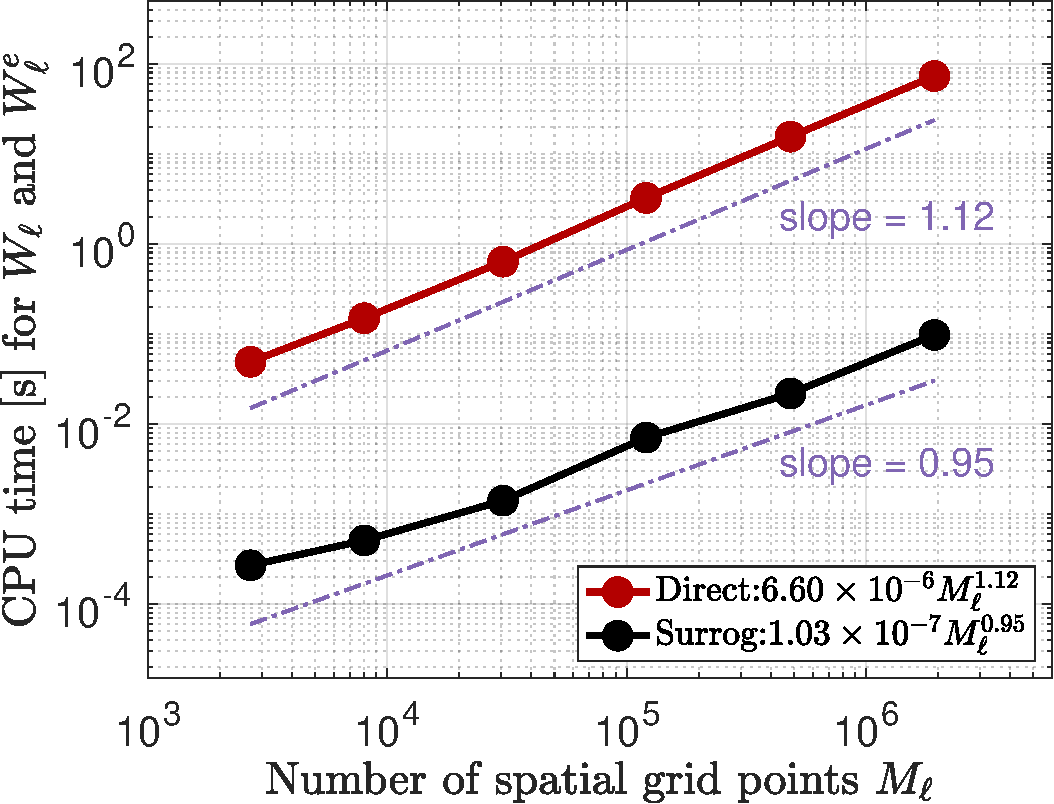
\includegraphics[height=0.36\linewidth]{./figures/CostPerSample_Ml.pdf}&
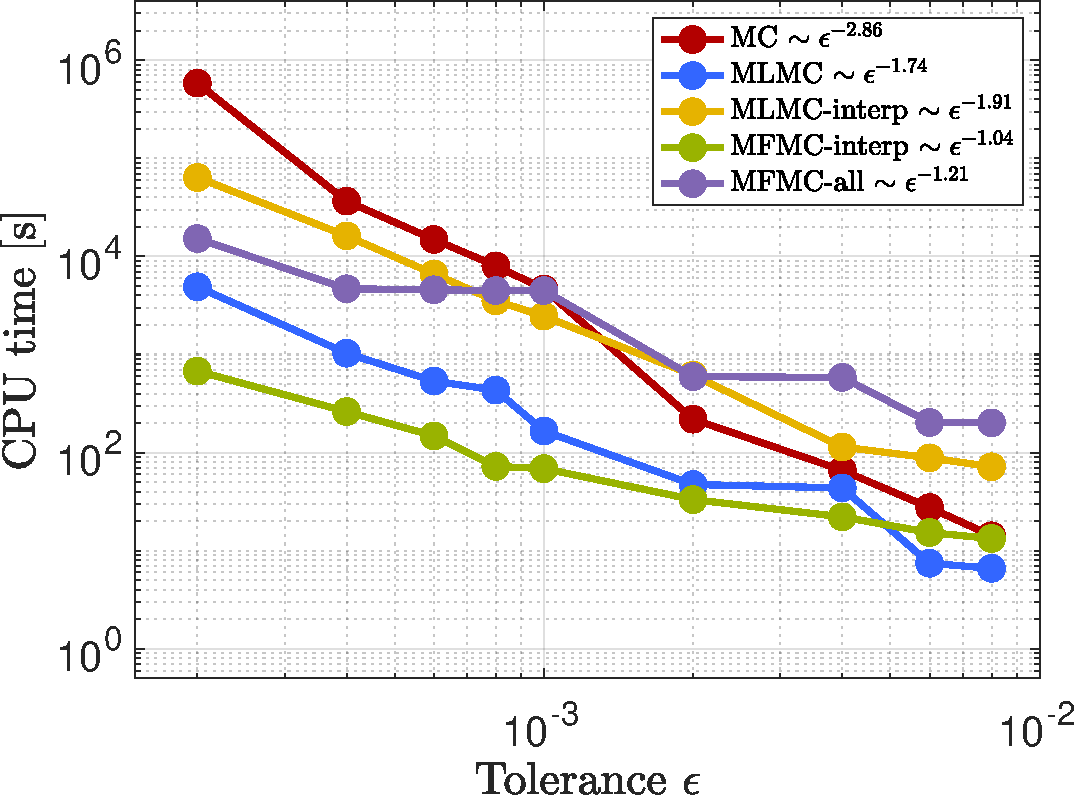
\includegraphics[height=0.36\linewidth]{./figures/Cost_epsilon.pdf}
\end{tabular}
\caption{Left:  Mean CPU times of 500 realizations of solutions for direct computations $W_\ell$ and surrogate evaluations $W_\ell^e$ vs.\ an increasing number of spatial grid points $M_\ell$ with $\ell = 0$ to 5. Right:  Total CPU time v.s. $\epsilon$ for simulation of various methods.}
\label{fig:CostEstimatePlot}
\end{figure}
%



 
 % While the offline preparation incurs non-negligible computational expenses, these costs are justified by the substantial savings achieved during large-scale online sampling, particularly in applications requiring thousands of high-fidelity model evaluations. As a one-time expense, the precomputed surrogates and statistical parameters are reused throughout the online phase, amortizing the initial overhead across all subsequent multi-fidelity Monte Carlo realizations.

%
\begin{table}[ht]
\centering
\scalebox{0.8}{
\begin{tabular}{c|c|c|c|c|c|c|c|c|c|c|c|c|c|c|c|c|c|c|}
\hline
\multicolumn{1}{|c|}{$\epsilon$} &$2\times 10^{-4}$&$4\times 10^{-4}\sim 1\times 10^{-3}$&$2\times 10^{-3} \sim 4\times 10^{-3}$&$6\times 10^{-3} \sim 8\times 10^{-3}$\\
\hline
\multicolumn{1}{|c|}{ Time to build surrogate }&2.39e+03&5.53e+02&1.08e+02&2.11e+01\\
\hline
\multicolumn{1}{|c|}{Time to estimate parameters}&1.21e+04&3.87e+03&4.54e+02&1.66e+02\\
% &2.02e+00&7.90e+00&3.10e+01&1.52e+02&8.12e+02&3.56e+03\\
\hline
\multicolumn{1}{|c|}{Samples required for dynamic sampling}& 30&50&30&50\\
\hline
\end{tabular}
}
\caption{Computational costs and sample requirements for low-fidelity model construction and parameter estimation. The second row: CPU time required to construct low-fidelity models $\widehat u_{h,k}$, generated using a sparse grid of level $q=1$ on coarser meshes than the high-fidelity model. The third row: CPU time for parameter estimation using a dynamic strategy with $\delta-0.01$. The last row: number of samples needed to compute the coefficients for each low-fidelity model.}
\label{Tab:Offline_cost}
\end{table}
%





% %
% \begin{table}[ht]
% \centering
% \scalebox{0.8}{
% \begin{tabular}{c|c|c|c|c|c|c|c|c|c|c|c|c|c|c|c|c|c|c|}
% \cline{1-7}	
% \multicolumn{1}{|c|}{$\ell$} &0&1&2&3&4&5\\
% \hline
% \multicolumn{1}{|c|}{$M_\ell$} &$2685$ &$8019$ &$30449$ &$120697$ &$484080$ &$1934365$\\
% \hline
% \multicolumn{1}{|c|}{Model $k$} &$\widehat u_{h,5}$&$\widehat u_{h,4}$&$\widehat u_{h,3}$&$\widehat u_{h,2}$&&\\
% \hline
% \multicolumn{1}{|c|}{$\rho_{1,k}$ (24 nodes), ref l=3}&0.9802&0.9958 &0.9976&0.9984&&\\
% \hline
% \multicolumn{1}{|c|}{$\sigma_{k}$}&9.3826e-05 &1.374e-04 &1.2405e-04 &1.2016e-04 &&\\
% \hline
% \multicolumn{1}{|c|}{Covariance} &1.0807e-04 &1.3283e-04 &1.2646e-04 &1.2457e-04 &&\\
% \hline
% \end{tabular}}
% \caption{$\epsilon = 4\times 10^{-3}\;\;\& \;\;2\times 10^{-3}$. High fidelity model: finite element solution on mesh with 120697 grid nodes. $\sigma_1 = 1.2955e-04$. The data are estimated using 500 samples. The selected models are $[\widehat u_{h,2},\widehat u_{h,4},\widehat u_{h,5}]$.}
% % \label{Tab:Dof}
% \end{table}
% %

% %
% \begin{table}[ht]
% \centering
% \scalebox{0.8}{
% \begin{tabular}{c|c|c|c|c|c|c|c|c|c|c|c|c|c|c|c|c|c|c|}
% \cline{1-7}	
% \multicolumn{1}{|c|}{$\ell$} &0&1&2&3&4&5\\
% \hline
% \multicolumn{1}{|c|}{$M_\ell$} &$2685$ &$8019$ &$30449$ &$120697$ &$484080$ &$1934365$\\
% \hline
% \multicolumn{1}{|c|}{Model $k$} &$\widehat u_{h,6}$&$\widehat u_{h,5}$&$\widehat u_{h,4}$&$\widehat u_{h,3}$&$\widehat u_{h,2}$&\\
% \hline
% \multicolumn{1}{|c|}{$\rho_{1,k}$ (24 nodes), ref l=3}&9.0103e-01 &9.2531e-01 &9.2415e-01 &9.2366e-01 &9.2307e-01 &\\
% \hline
% \multicolumn{1}{|c|}{$\sigma_{k}$}&1.1064e-04 &1.3571e-04 &1.2930e-04 &1.2757e-04  &1.2742e-04  &\\
% \hline
% \multicolumn{1}{|c|}{Covariance}&8.9789e-05 &1.2808e-04 &1.1657e-04 &1.1358e-04 &1.1346e-04 &\\
% \hline
% \end{tabular}}
% \caption{$\epsilon = 1\times 10^{-3}\;\;\& \;\;8\times 10^{-4}\;\;\& \;\;6\times 10^{-4}\;\;\& \;\;4\times 10^{-4}$. High fidelity model: finite element solution on mesh with 484080 grid nodes. $\sigma_1 = 1.6794e-04$. The data are estimated using 500 samples.}
% % \label{Tab:Dof}
% \end{table}
% %

% %
% \begin{table}[ht]
% \centering
% \scalebox{0.8}{
% \begin{tabular}{c|c|c|c|c|c|c|c|c|c|c|c|c|c|c|c|c|c|c|}
% \cline{1-7}	
% \multicolumn{1}{|c|}{$\ell$} &0&1&2&3&4&5\\
% \hline
% \multicolumn{1}{|c|}{$M_\ell$} &$2685$ &$8019$ &$30449$ &$120697$ &$484080$ &$1934365$\\
% \hline
% \multicolumn{1}{|c|}{Model $k$} &$\widehat u_{h,7}$&$\widehat u_{h,6}$&$\widehat u_{h,5}$&$\widehat u_{h,4}$&$\widehat u_{h,3}$&$\widehat u_{h,2}$\\
% % \hline
% % \multicolumn{1}{|c|}{$C_k$ direct solve}&1.2029e+02&2.6478e+01&5.3710e+00&1.1269e+00&2.9300e-01&9.6419e-02\\
% % \hline
% % \multicolumn{1}{|c|}{$C_k$ surrog evaluation(24 nodes)}&1.2595e-01&2.9694e-02&9.1085e-03&3.0580e-03&1.1869e-03&2.5127e-04\\
% \hline
% \multicolumn{1}{|c|}{$\rho_{1,k}$ (24 nodes), ref l=3}&1.0095e+00   &1.0092e+00   &1.0095e+00   &1.0090e+00   &1.0091e+00   &9.9033e-01\\
% \hline
% \multicolumn{1}{|c|}{$\sigma_{k}$}&1.2775e-04   &1.2804e-04   &1.2796e-04   &1.3161e-04   &1.4586e-04   &9.7734e-05\\
% \hline
% \multicolumn{1}{|c|}{Covariance}&1.3872e-04   &1.3885e-04   &1.3884e-04   &1.4073e-04   &1.4817e-04   &1.1903e-04\\
% \hline
% \end{tabular}}
% \caption{$\epsilon = 2\times 10^{-4}$. High fidelity model: finite element solution on mesh with 1934365 grid nodes. $\sigma_1 = 1.4782e-04$. The data are estimated using 100 samples. Total time: 1.6676e+04  + 1.5951e+04 +  1.6914e+04 + 1.7699e+04 +  1.7657e+04 + 1.7683e+04}
% % \label{Tab:Dof}
% \end{table}
% % 



% =============================
\subsection{Sampling (online) cost}
% =============================
After completing the offline procedure, the necessary statistical parameters and selected low-fidelity models are obtained to estimate the MFMC estimator in the online phase. In the theoretical formulation of the MFMC estimator \eqref{eq:MFMC_estimator_independent}, the weights $\alpha_k $are assumed to be deterministic and optimally chosen, ensuring that the estimator remains unbiased. This follows from the expectation property $\mathbb{E}(\alpha_k Y_k) = \alpha_k \mathbb{E}(Y_k)$ and $\mathbb{E}(Y_k) = 0$ for $k=2,\ldots, K$. However, in practical implementations, if the same samples are reused for both parameter estimation and the online sampling of $A^{\text{MF}}$, the weights $\alpha_k$ become random variables that depend on the sample set, leading to a correlation between $\alpha_k$  and the correction term $Y_k$. Consequently, this introduces a bias in the estimator, as $\mathbb{E}(\alpha_k Y_k) = \mathbb{E}(\alpha_k Y_k)-\mathbb{E}(\alpha_k)\mathbb{E}(Y_k) = \text{Cov}(\alpha_k,Y_k)\neq 0$, resulting in $\mathbb{E}(A^{\text{MF}})\neq \mathbb{E}(Y_1)$. To maintain the unbiasedness of the MFMC estimator, the samples used for parameter estimation must be statistically independent from those used in the online sampling process, ensuring that $\alpha_k$ and $Y_k$ remain uncorrelated. If reusing offline samples is unavoidable, the sample size should be sufficiently large to ensure that the estimated $\alpha_k$  values closely approximate their theoretical counterparts, thereby minimizing any induced bias.


  
After the offline procedure, we obtain the necessary statistical parameters and selected low-fidelity models for estimating the MFMC estimator in the online process. In \eqref{eq:MFMC_estimator_independent}, if the weights $\alpha_k$ are deterministic (theoretically optimal), the estimator is unbiased since $\mathbb{E}(\alpha_k Y_k) = \alpha_k \mathbb{E}(Y_k)$ and $\mathbb{E}(Y_k) = 0$ for $k=2,\ldots, K$. However, if we reuse samples for parameter estimation with those used in the online sampling for $A^{\text{MF}}$, the weights $\alpha_k$ become random variables dependent on the samples and correlated with the correction term $Y_k$. This results in $\mathbb{E}(\alpha_k Y_k) = \mathbb{E}(\alpha_k Y_k)-\mathbb{E}(\alpha_k)\mathbb{E}(Y_k) = \text{Cov}(\alpha_k,Y_k)\neq 0$ and $\mathbb{E}(A^{\text{MF}})\neq \mathbb{E}(Y_1)$, introducing bias into the MFMC estimator. To preserve unbiasedness, samples for parameter estimation must be statistically independent from those used in online sampling. This ensures that $\alpha_k$ and $Y_k$ remain uncorrelated. If offline samples must be reused, their sample size should be sufficiently large to approximate theoretical values of  $\alpha_k$.

The right plot in Figure \ref{fig:CostEstimatePlot} illustrates the sampling cost, showing that the CPU time for MFMC scales as $\epsilon^{-1.09}$, consistent with Theorem \ref{thm:Sample_cost_est}. For instance, when $\epsilon=2\times 10^{-4}$, the term $\sqrt{C_1(\rho_{1,1}^2-\rho_{1,2}^2)}$ is 0.191, while $\sum_{k=2}^K\sqrt{C_k(\rho_{1,k}^2-\rho_{1,k+1}^2)}$ is 0.0239, indicating that the high-fidelity model cost dominates that of all low-fidelity models combined. Since the cost of  high-fidelity model scales as $\epsilon^{\frac{\beta-\gamma}{2\alpha}}$,  the total MFMC sampling cost  $\mathcal{W}^{\text{MF}}$ follows $\epsilon^{-2+\frac{\beta-\gamma}{\alpha}}$. Given \cite{ElLiSa:2023,ElLiSa:2025} estimates $\beta\approx 2, \alpha\approx 1$, and from the left plot of Figure \ref{fig:CostEstimatePlot}, $\gamma\approx 1.1$, we obtain $\mathcal{W}^{\text{MF}}\sim \epsilon^{-1.09}$, aligning with the experimental results. The cost of the Monte Carlo approach scales as $\epsilon^{-2-\gamma/\alpha}\approx \mathcal{O}(\epsilon^{-3.1})$. The cost of the multilevel Monte Carlo approach scales as $\epsilon^{-2}$.

The purple curve in the plot represents the total online and offline costs of MFMC. When $\epsilon$ is above $10^{-3}$, MFMC incurs higher costs than MC due to the estimation of  statistical parameters. However, as $\epsilon$ decreases, MFMC outperforms both MC and MLMC with interpolation in overall efficiency. The speed up of different methods compared to the MC benchmark is shown in Table \ref{Tab:CPU_time}, the speed up reflect the inverse of cost efficiency. But this speed up deviate from the cost efficiency in Table \ref{Tab:MFMC_parameters} and Table \ref{Tab:MFMC_parameters_dynamic} due to extra cost associated with interpolation, and some computational overhead.


%
\begin{table}[ht]
	\centering
			\scalebox{0.62}{
   \begin{tabular}{c|c|c|c|c|c|c|c|c|c|c|c|c|}
			\hline
			\multicolumn{1}{|c|}{ }&MC-FE &MLMC-FE&MLMC-FE(Interp)
            % &MFMC-FE 
            &MFMC-FE(Interp)&MFMC-FE(Interp)+upfront\\
			\multicolumn{1}{|c|}{$\epsilon$}&Time &\begin{tabular}{cc} \,\,\,\,\,Time & \,\,\,Speedup \end{tabular}&\begin{tabular}{cc} \,\,\,\,Time & \,\,\,Speedup \end{tabular} &\begin{tabular}{cc} \,\,\,\,Time & \,\,\,Speedup \end{tabular} &\begin{tabular}{cc} \,\,\,\,Time & \,\,\,Speedup \end{tabular}\\
            % &\begin{tabular}{cc} \,\,\,\,Time & \,\,\,Speedup \end{tabular}\\
			\hline
			\multicolumn{1}{|c|}{$8\times 10^{-3} $}&1.42e+01&\begin{tabular}{cc}6.61e+00\,\,\, & 2.1 \end{tabular}&\begin{tabular}{cc}7.17e+01\,\,  &0.2\end{tabular}
            % &\begin{tabular}{cc}7.2998e+00\,\,  &1.9453e+00 \end{tabular} 
            &\begin{tabular}{cc}1.33e+01\,\,   &1.1 \end{tabular} &\begin{tabular}{cc}2.01e+02\,\,  &0.07\end{tabular}\\
			\multicolumn{1}{|c|}{$6\times 10^{-3} $}&2.75e+01&\begin{tabular}{cc}7.44e+00\,\,\, & 3.7 \end{tabular}&\begin{tabular}{cc}8.84e+01\,\,  &0.3\end{tabular}
            % &\begin{tabular}{cc}9.3266e+00\,\, &2.9486e+00 \end{tabular}
            &\begin{tabular}{cc}1.53e+01&1.8
            \end{tabular}&\begin{tabular}{cc}2.03e+02\,\,  &0.1\end{tabular}\\
			\multicolumn{1}{|c|}{$4\times 10^{-3} $}&6.60e+01&\begin{tabular}{cc}4.36e+01\,\,\, & 1.5 \end{tabular}&\begin{tabular}{cc}1.14e+02\,\,  &0.6\end{tabular}
            % &\begin{tabular}{cc}1.9119e+01&3.4521e+00\end{tabular}
            &\begin{tabular}{cc}2.21e+01&3.0
            \end{tabular}&\begin{tabular}{cc}5.84e+02\,\,  &0.1\end{tabular}\\
			\multicolumn{1}{|c|}{$2\times 10^{-3} $}&2.19e+02&\begin{tabular}{cc}4.73e+01\,\, & 4.6\end{tabular}&\begin{tabular}{cc}6.16e+02\,\,  &0.4\end{tabular}
            % &\begin{tabular}{cc}3.0242e+01& 7.2416e+00\end{tabular}
            &\begin{tabular}{cc}3.32e+01&6.6 \end{tabular}&\begin{tabular}{cc}5.95e+02\,\,  &0.4\end{tabular}\\
			\multicolumn{1}{|c|}{$10^{-3} $}&4.66e+03&\begin{tabular}{cr}1.66e+02\,\, & 28.1 \end{tabular}&\begin{tabular}{cc}2.46e+03\,\,  &1.9\end{tabular}
            % &\begin{tabular}{cc}6.5732e+01&7.0894e+01\end{tabular}
            &\begin{tabular}{cc}6.87e+01&67.9
            \end{tabular}&\begin{tabular}{cc}4.49e+03\,\,  &1.0\end{tabular}\\
			\multicolumn{1}{|c|}{$8\times 10^{-4} $}&8.02e+03&\begin{tabular}{cc}4.33e+02\,\, & 18.5 \end{tabular}&\begin{tabular}{cc}3.53e+03\,\,  &2.3\end{tabular}
            % &\begin{tabular}{cc}6.9345e+01&1.1565e+02\end{tabular}
            &\begin{tabular}{cc}7.23e+01&111.0
            \end{tabular}&\begin{tabular}{cc}4.49e+03\,\,  &1.8\end{tabular}\\
			\multicolumn{1}{|c|}{$6\times 10^{-4} $}&1.49e+04&\begin{tabular}{cc}5.36e+02\,\, & 27.8 \end{tabular}&\begin{tabular}{cc}6.63e+03\,\,  &2.2\end{tabular}
            % &\begin{tabular}{cc}1.4482e+02&1.0289e+02\end{tabular}
            &\begin{tabular}{cc}1.48e+02&100.6
            \end{tabular}&\begin{tabular}{cc}4.57e+03\,\,  &3.3\end{tabular}\\
                \multicolumn{1}{|c|}{$4\times 10^{-4} $}&3.66e+04&\begin{tabular}{cc}1.03e+03\,\, & 35.4 \end{tabular}&\begin{tabular}{cc}1.62e+04\,\,  &2.3\end{tabular} &\begin{tabular}{cc}2.62e+02&139.7 \end{tabular}
                % &\begin{tabular}{cc}2.6595e+02&1.3762e+02\end{tabular}
            &\begin{tabular}{cc}4.68e+03\,\,  &7.8\end{tabular}\\
                \multicolumn{1}{|c|}{$2\times 10^{-4} $}&5.84e+05$^{\ast}$\!\!\!&\begin{tabular}{cc}4.90e+03 &119.2 \end{tabular} &\begin{tabular}{cc}6.38e+04\,\,  &9.2\end{tabular}
                % &\begin{tabular}{cc} 6.6985e+02&8.7184e+02 \end{tabular}
                &\begin{tabular}{cc}6.78e+02 &861.2 \end{tabular}&\begin{tabular}{cc}1.52e+04\,\,  &38.4\end{tabular}\\
			\hline
	\end{tabular}
 }
	\caption{The CPU time in seconds for MC-FE (left), MLMC-FE (middle left), MLMC-FE (middle) with interpolation to a common grid of level $\ell=4$, MFMC-FE (middle right) with interpolation to a common grid of level $\ell=4$,  and MFMC-FE (right) with interpolation to a common grid of level $\ell=4$ and the offline costs, together with speedups for the multi-fidelity methods, for a variety of choices of $\epsilon$. The computational cost associated with a tolerance of $\epsilon = 2\times 10^{-4}$ for Monte Carlo was prohibitive; the entry in the table for this tolerance (with an asterisk) is an estimate.}
	\label{Tab:CPU_time}
\end{table}
%

The sample size estimation for various $\epsilon$ is shown in Table \ref{Tab:SampleSize}. We first observe that the correspondence between the required finest spatial grid level as the corresponding tolerance decreases. Moreover, for the sample size estimation, we require a minimum of two samples for each level and each model for all methods. We observe that the MFMC requires much more sample size for the low fidelity models compared to both MC and MLMC.


%
\begin{table}[ht]
	\centering
			\scalebox{0.62}{
   \begin{tabular}{c|c|c|c|c|c|c|c|c|c|c|c|c|}
	    \cline{2-7}	
		&\multicolumn{6}{|c|}{ Level $\ell$}\\
			\hline
			\multicolumn{1}{|c|}{$\epsilon$}&0&1&2&3&4&5\\
			\hline
			\multicolumn{1}{|c|}{$8\times 10^{-3} $}&&&5&&&\\
			\multicolumn{1}{|c|}{$6\times 10^{-3} $}&&&9&&&\\
			\multicolumn{1}{|c|}{$4\times 10^{-3} $}&&&&21&&\\
			\multicolumn{1}{|c|}{$2\times 10^{-3} $}&&&&73&&\\
			\multicolumn{1}{|c|}{$10^{-3} $}&&&&&287&\\
			\multicolumn{1}{|c|}{$8\times 10^{-4} $}&&&&&445&\\
			\multicolumn{1}{|c|}{$6\times 10^{-4} $}&&&&&845&\\
                \multicolumn{1}{|c|}{$4\times 10^{-4} $}&&&&&2000&\\
                \multicolumn{1}{|c|}{$2\times 10^{-4} $}&&&&&& 8000$^{\ast}$\!\!\\
			\hline
	\end{tabular}
 \qquad
		\begin{tabular}{c|c|c|c|c|c|c|c|c|c|c|c|c|}
	    \cline{2-7}	
		&\multicolumn{6}{|c|}{ Level $\ell$}\\
			\hline
			\multicolumn{1}{|c|}{$\epsilon$}&0&1&2&3&4&5\\
			\hline
			\multicolumn{1}{|c|}{$8\times 10^{-3} $}&10     &2     &2&&&\\
			\multicolumn{1}{|c|}{$6\times 10^{-3} $}&12     &2     &2&&&\\
			\multicolumn{1}{|c|}{$4\times 10^{-3} $}&22     &5     &2     &2&&\\
			\multicolumn{1}{|c|}{$2\times 10^{-3} $}&163    &26     &5     &2&&\\
			\multicolumn{1}{|c|}{$10^{-3} $}&577   &90    &15     &3     &2&\\
			\multicolumn{1}{|c|}{$8\times 10^{-4} $}&1036 &157 &26 &5 &2&\\
			\multicolumn{1}{|c|}{$6\times 10^{-4} $}&1744 &266 &44 &9 &2&\\
                \multicolumn{1}{|c|}{$4\times 10^{-4} $}&3911 &553 &86 &17 &4&\\
                \multicolumn{1}{|c|}{$2\times 10^{-4} $}&15619 &2298 &370 &57 &12 &2\\
			\hline
	\end{tabular}
 \qquad
		\begin{tabular}{c|c|c|c|c|c|c|c|c|c|c|c|c|c|c|c|c|c|}
	    \cline{2-7}	
		&\multicolumn{6}{|c|}{ Level $\ell$}\\
			\hline
			\multicolumn{1}{|c|}{$\epsilon$}&0&1&2&3&4&5\\
			\hline
			\multicolumn{1}{|c|}{$8\times 10^{-3} $}&24&4&2&&&\\
			\multicolumn{1}{|c|}{$6\times 10^{-3} $}&43&7&2&&&\\
			\multicolumn{1}{|c|}{$4\times 10^{-3} $}&95&12&4&2&&\\
			\multicolumn{1}{|c|}{$2\times 10^{-3} $}&380&46&13&2&&\\
			\multicolumn{1}{|c|}{$10^{-3} $}&2444&301&79&13&2&\\
			\multicolumn{1}{|c|}{$8\times 10^{-4} $}&3819&470&123&21&2&\\
                \multicolumn{1}{|c|}{$6\times 10^{-4} $}&6788&835&218&36&2&\\
			\multicolumn{1}{|c|}{$4\times 10^{-4} $}&15273&1879&489&81&2&\\
                \multicolumn{1}{|c|}{$2\times 10^{-4} $}&97028&13374&2544&335&-&5\\
			\hline
	\end{tabular}
 
 }
	\caption{The optimal sample size estimation for MC-FE (left), uniform MLMC-FE (middle), and MFMC-FE (right). The simulations were conducted for a variety of choices of $\epsilon$. The computational cost associated with a tolerance of $\epsilon = 2\times 10^{-4}$ for Monte Carlo was prohibitive; the entry in the table for this tolerance (with an asterisk) is an estimate.}
	\label{Tab:SampleSize}
\end{table}
%


% \JLcolor{According to \cite{PeGuWi:2018}, pages A3174 and A3181–A3182, perturbations in the sample variance and sample correlation coefficients have a small impact on the overall sample size and computational work. However, from my perspective, inaccurate estimation of these statistical parameters can also affect the model selection process. If these statistics are not reliably computed, low-fidelity models with misleading characteristics may be selected or rejected incorrectly, potentially undermining the efficiency and accuracy of the MFMC framework. In particular, models that exhibit inconsistent statistical properties violating the two conditions in Theorem \ref{thm:Sample_size_est} could be included, leading to suboptimal model choices for the low-fidelity approximations and, consequently, affecting the overall performance of the multi-fidelity estimator.}






% =============================
\subsection{Properties of geometric discriptors}
% =============================
As demonstrated in \cite{ElLiSa:2023}, multilevel Monte Carlo (MLMC) implementations face significant challenges when dealing with plasma boundary distortions caused by extrapolation errors during cross-level sample correction aggregation on non-nested, geometry-conforming meshes. These errors arise from mismatches in spatial resolution when coarse-grid corrections are accumulated across multiple levels. This distortion can be mitigated by interpolating the multilevel solutions onto a unified fine grid with level $\ell=5$, effectively reconciling resolution disparities while preserving the geometric fidelity of the plasma boundary. Similarly, in the multi-fidelity Monte Carlo (MFMC) approach, sample corrections for various low-fidelity models are generated using stochastic collocation on the same non-nested, uniform, geometry-conforming coarse grids. To ensures that all corrections are aligned on a consistent spatial resolution for generating the multi-fidelity estimator for the expected plasma field in \eqref{eq:QoI}, it is necessary to project these corrections onto a common fine mesh, enabling accurate and reliable estimation of the quantity of interest. Figure \ref{fig:QoI_plot} shows the contour plot of plasma boundary of the \eqref{eq:QoI} for Monte Carlo, multilevel Monte Carlo and multi-fidelity Monte Carlo samplings. We observe that the plasma boundary resulting from the multi-fidelity Monte Carlo behaves in a similar fashion as that in the benchmark boundary sampled with Monte Carlo.

%=====================================================================================
\noindent \textbf{Plasma boundary.} 
%=====================================================================================






% %
% \begin{table}[ht]
% \centering
% \scalebox{0.8}{
% \begin{tabular}{c|c|c|c|c|c|c|c|c|c|c|c|c|c|c|c|c|c|c|}
% \cline{1-7}	
% \multicolumn{1}{|c|}{Dof} &$1934365$&$484080$&$120697$&$30449$&$8019$&$2685$\\
% \hline
% \multicolumn{1}{|c|}{Model $k$} &$f_1$&$f_2$&$f_3$&$f_4$&$f_5$&$f_6$\\
% % \hline
% % \multicolumn{1}{|c|}{$C_k$ direct solve}&1.2029e+02&2.6478e+01&5.3710e+00&1.1269e+00&2.9300e-01&9.6419e-02\\
% % \hline
% % \multicolumn{1}{|c|}{$C_k$ surrog evaluation(24 nodes)}&1.2595e-01&2.9694e-02&9.1085e-03&3.0580e-03&1.1869e-03&2.5127e-04\\
% \hline
% \multicolumn{1}{|c|}{$\rho_{1,k}$ (24 nodes), ref l=3}&&&&0.9678&0.9670&0.9488\\
% \hline
% \multicolumn{1}{|c|}{$\sigma_{k}$}&&&&1.1696e-04&1.2929e-04&8.8977e-05\\
% \hline
% \multicolumn{1}{|c|}{Covariance}&&&&1.3065e-04&1.3726e-04&1.1172e-04\\
% \hline
% \end{tabular}}
% \caption{High fidelity model: finite element solution on mesh with 30449 grid nodes. $\sigma_1 = 1.5582e-04$. The data are estimated using 500 samples.}
% % \label{Tab:Dof}
% \end{table}
% %









   

   


\begin{figure}[ht!]\centering
\begin{tabular}{ccc}
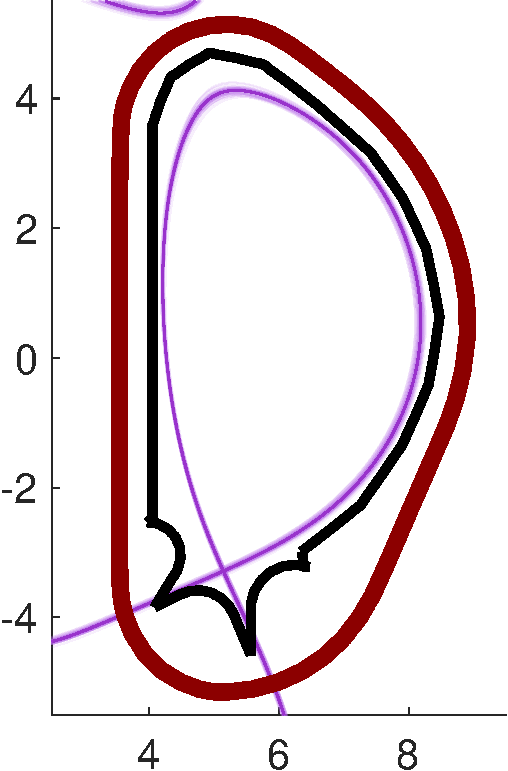
\includegraphics[width=0.19\linewidth]{./figures/QoI_MC_uniform.pdf}
% &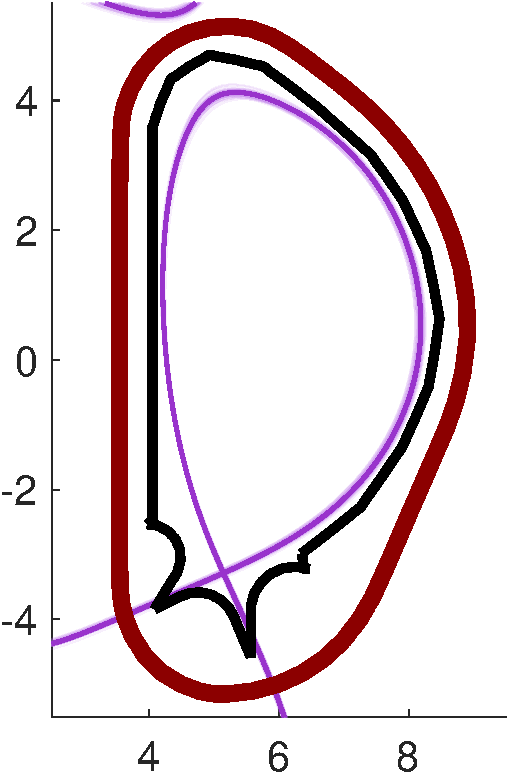
\includegraphics[width=0.19\linewidth]{./figures/QoI_MC_surrogate.pdf}
&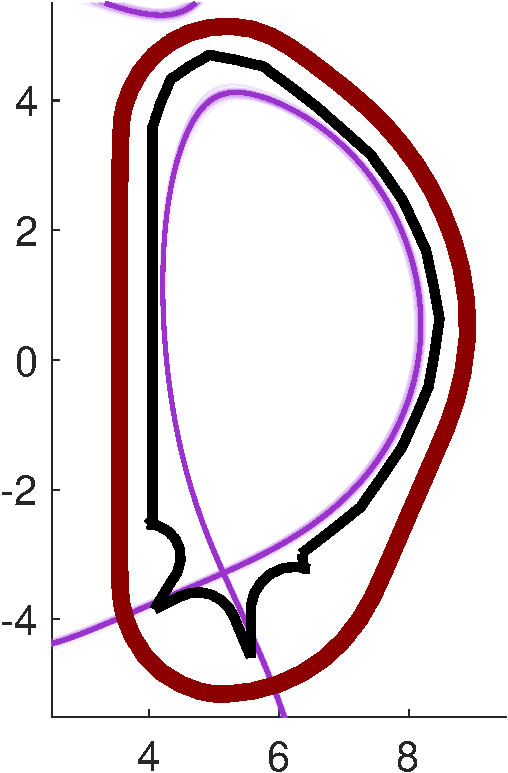
\includegraphics[width=0.19\linewidth]{./figures/QoI_MLMC_DirectSolver_Interp2CommonGrid.pdf} 
& 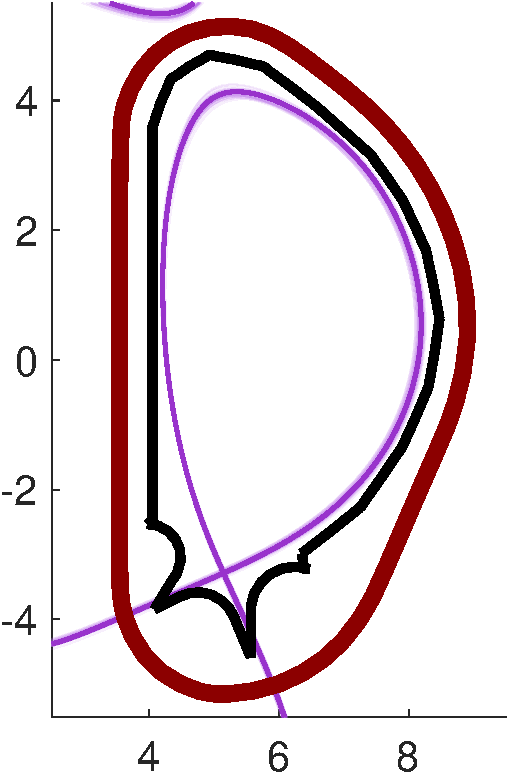
\includegraphics[width=0.19\linewidth]{./figures/QoI_MFMC.pdf} 
\\
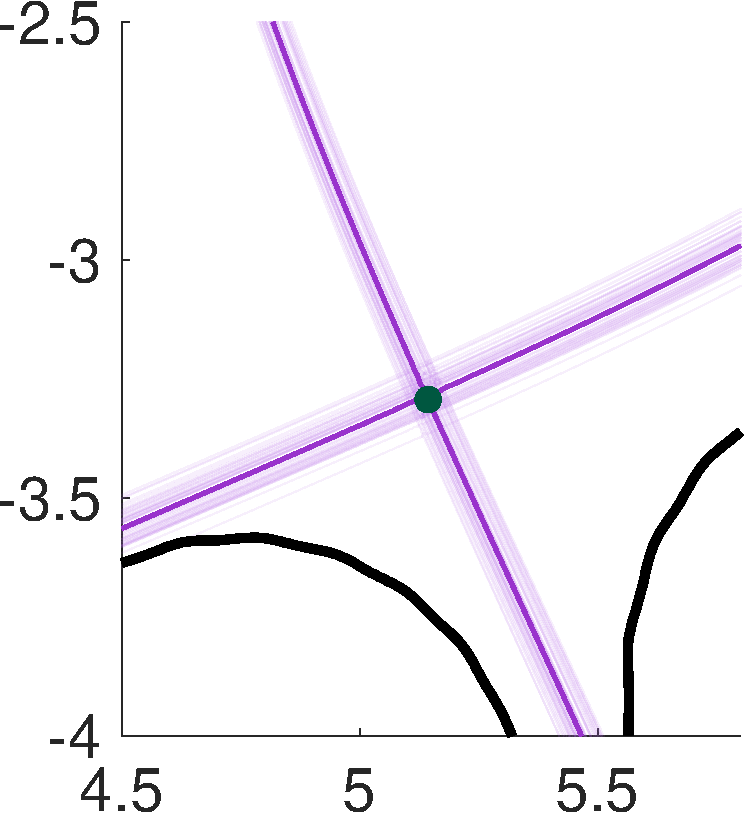
\includegraphics[width=0.19\linewidth]{./figures/QoI_MC_uniform_xptRegion.pdf} 
% &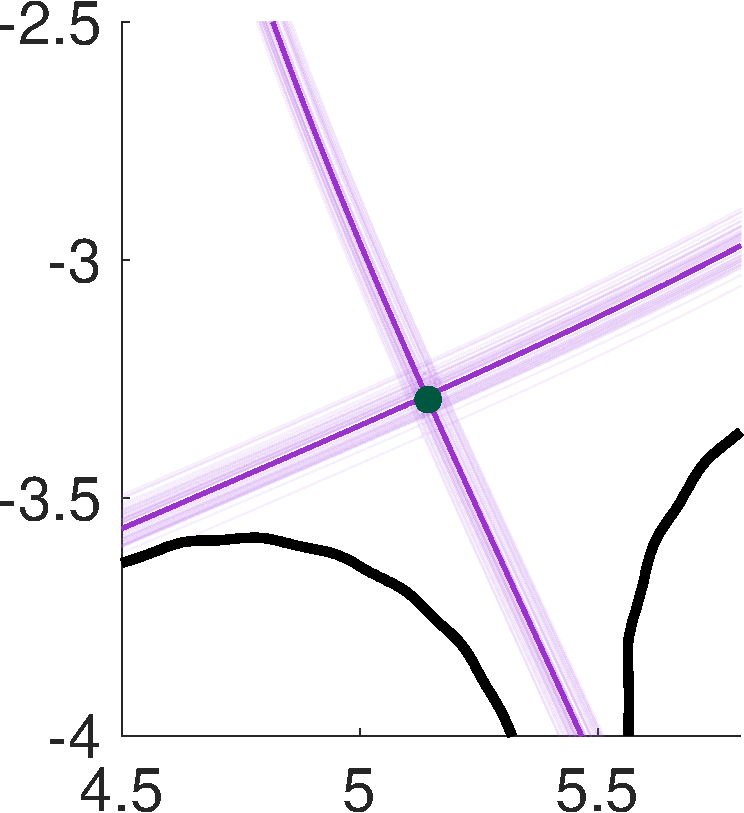
\includegraphics[width=0.19\linewidth]{./figures/QoI_MC_surrogate_xptRegion.pdf}
&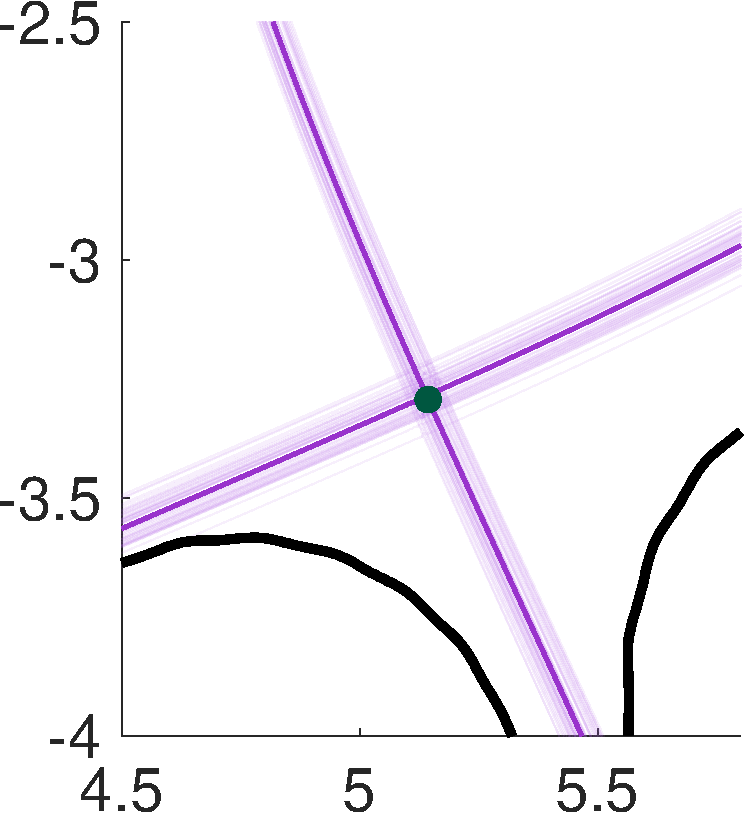
\includegraphics[width=0.19\linewidth]{./figures/QoI_MLMC_DirectSolver_xptRegion_Interp2CommonGrid.pdf} 
&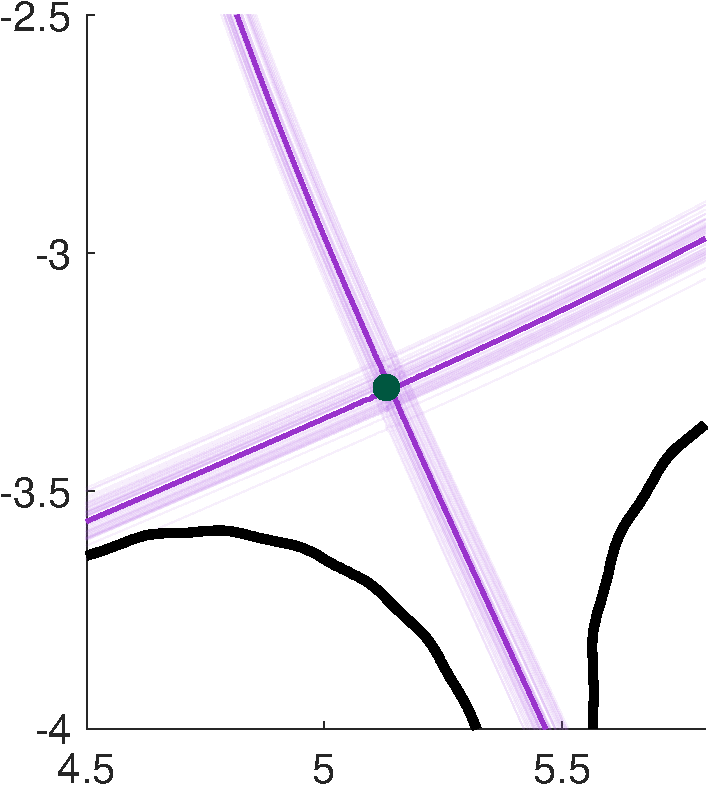
\includegraphics[width=0.19\linewidth]{./figures/QoI_MFMC_xptRegion.pdf} 
\\[1ex]
\quad MC-FE &MLMC-FE (Interp) &MFMC-FE (Interp) \\[-0.5ex]
\end{tabular}
\caption{The overlayed plasma boundaries of 50 random realizations are 
displayed in the top row as violet curves (interpolated to the finest mesh with spatial grid level $\ell=4$). The solid violet line is the plasma boundary of the expected 
poloidal flux generated with tolerance $\epsilon=4\times 10^{-4}$. 
The inner and outer walls of the reactor are displayed in solid black and 
dark red respectively. The bottom row shows the regions close to the 
x-points in more detail. The dark green dots are the x-points of the expected 
solution. The columns from left to right correspond to simulations using the 
MC-FE approach, MLMC-FE and MFMC-FE. All simulations were interpolated to the geometry-conforming uniform meshes of discretization level $\ell=4$.} 
\label{fig:QoI_plot}
\end{figure}
%












\noindent \textbf{Geometric descriptors.}
%
\begin{table}[ht]
	\centering
			\scalebox{0.6}{
		\begin{tabular}{c|c|c|c|c|c|c|}
			\cline{2-5}
				&\multicolumn{1}{c|}{MC-FE}&MLMC-FE&MLMC-FE (Interp)&MFMC-FE (Interp)\\
			\hline
			\multicolumn{1}{|c|}{x point}&(5.14,-3.29)&(5.14,-3.29)&(5.14,-3.29)&(5.14,-3.29)\\
			\hline
			\multicolumn{1}{|c|}{magnetic axis}&(6.41,0.61)&(6.44,0.56)&(6.41,0.61)&(6.41,0.61)\\
			\hline
			\multicolumn{1}{|c|}{strike} &(4.16,-3.71)&(4.16,-3.71)&(4.16,-3.71)&(4.16,-3.71)\\
			\multicolumn{1}{|c|}{points}&(5.56,-4.22)&(5.56,-4.22)&(5.56,-4.22)&(5.56,-4.22)\\
			\hline
			\multicolumn{1}{|c|}{inverse aspect ratio} &0.32&0.32&0.32&0.32\\
			\hline
			\multicolumn{1}{|c|}{elongation} &1.86&1.87&1.86&1.86\\
			\hline
			\multicolumn{1}{|c|}{upper triangularity}&0.43&0.43&0.43&0.43\\
			\hline
			\multicolumn{1}{|c|}{lower triangularity} &0.53&0.53&0.53&0.53\\
			\hline
	\end{tabular}
  }
	\caption{Geometric parameters of the expected poloidal flux $u$ from MC-FE with direct solver, MLMC-FE with direct solver,  MLMC-FE with direct solver with interpolating solution to a common fine grid of level $L=5$, MFMC-FE with surrogate with interpolating solution to a common fine grid of level $L=5$. The results are generated with an nMSE $4\times 10^{-4}$ on the geometry-conforming uniform mesh set.}
	\label{Tab: QoI_GeoInfo}
\end{table}






% % =============================
% \subsection{Uncertainties in the source term}
% % =============================
% In this experiment, we study the uncertainty in perturbing the reference parameter that characterizes the source term \eqref{eq:source}.
% \begin{table}[ht]
% 	\centering
% 			\scalebox{0.62}{
%    \begin{tabular}{c|c|c|c|c|c|c|c|c|c|c|c|c|}
% 	    \cline{2-7}	
% 		&\multicolumn{6}{|c|}{ Level $\ell$}\\
% 			\hline
% 			\multicolumn{1}{|c|}{$\epsilon$}&0&1&2&3&4&5\\
% 			\hline
% 			\multicolumn{1}{|c|}{$8\times 10^{-3} $}&&&8&&&\\
% 			\multicolumn{1}{|c|}{$6\times 10^{-3} $}&&&10&&&\\
% 			\multicolumn{1}{|c|}{$4\times 10^{-3} $}&&&&25&&\\
% 			\multicolumn{1}{|c|}{$2\times 10^{-3} $}&&&&93&&\\
% 			\multicolumn{1}{|c|}{$10^{-3} $}&&&&&423&\\
% 			\multicolumn{1}{|c|}{$8\times 10^{-4} $}&&&&&678&\\
% 			\multicolumn{1}{|c|}{$6\times 10^{-4} $}&&&&&1211&\\
%                 \multicolumn{1}{|c|}{$4\times 10^{-4} $}&&&&&2700$^{\ast}$&\\
%                 \multicolumn{1}{|c|}{$2\times 10^{-4} $}&&&&&&11000$^{\ast}$\!\!\\
% 			\hline
% 	\end{tabular}
%  \qquad
% 		\begin{tabular}{c|c|c|c|c|c|c|c|c|c|c|c|c|}
% 	    \cline{2-7}	
% 		&\multicolumn{6}{|c|}{ Level $\ell$}\\
% 			\hline
% 			\multicolumn{1}{|c|}{$\epsilon$}&0&1&2&3&4&5\\
% 			\hline
% 			\multicolumn{1}{|c|}{$8\times 10^{-3} $}&10 &2 &2&&&\\
% 			\multicolumn{1}{|c|}{$6\times 10^{-3} $}&11 &3 &2 &&&\\
% 			\multicolumn{1}{|c|}{$4\times 10^{-3} $}&33 &7 &2 &2&&\\
% 			\multicolumn{1}{|c|}{$2\times 10^{-3} $}&150 &27 &4 &2&&\\
% 			\multicolumn{1}{|c|}{$10^{-3} $}&692 &116 &19 &4 &2&\\
% 			\multicolumn{1}{|c|}{$8\times 10^{-4} $}&1008 &160 &27 &6 &2&\\
% 			\multicolumn{1}{|c|}{$6\times 10^{-4} $}&2022 &322 &53 &10 &3&\\
%                 \multicolumn{1}{|c|}{$4\times 10^{-4} $}&4158 &613 &106 &14 &4&\\
%                 \multicolumn{1}{|c|}{$2\times 10^{-4} $}&17158 &2612 &442 &59 &13 &2\\
% 			\hline
% 	\end{tabular}
%  \qquad
% 		\begin{tabular}{c|c|c|c|c|c|c|c|c|c|c|c|c|c|c|c|c|c|}
% 	    \cline{2-7}	
% 		&\multicolumn{6}{|c|}{ Level $\ell$}\\
% 			\hline
% 			\multicolumn{1}{|c|}{$\epsilon$}&0&1&2&3&4&5\\
% 			\hline
% 			\multicolumn{1}{|c|}{$8\times 10^{-3} $}&&&&&&\\
% 			\multicolumn{1}{|c|}{$6\times 10^{-3} $}&&&&&&\\
% 			\multicolumn{1}{|c|}{$4\times 10^{-3} $}&&&\\
% 			\multicolumn{1}{|c|}{$2\times 10^{-3} $}&&&\\
% 			\multicolumn{1}{|c|}{$10^{-3} $}&&&&&&\\
% 			\multicolumn{1}{|c|}{$8\times 10^{-4} $}&&&&&&\\
%                 \multicolumn{1}{|c|}{$6\times 10^{-4} $}&&&&&&\\
% 			\multicolumn{1}{|c|}{$4\times 10^{-4} $}&&&&&&\\
%                 \multicolumn{1}{|c|}{$2\times 10^{-4} $}&&&&&&\\
% 			\hline
% 	\end{tabular}
 
%  }
% 	\caption{The optimal sample size estimation for MC-FE (left), uniform MLMC-FE (middle), and MFMC-FE (right). The simulations were conducted for a variety of choices of $\epsilon$. The computational cost associated with a tolerance of $\epsilon = 2\times 10^{-4}$ for Monte Carlo was prohibitive; the entry in the table for this tolerance (with an asterisk) is an estimate.}
% 	\label{Tab:SampleSize_Source_Term}
% \end{table}

% \begin{table}[ht]
% 	\centering
% 			\scalebox{0.62}{
%    \begin{tabular}{c|c|c|c|c|c|c|c|c|c|c|c|c|}
% 			\hline
% 			\multicolumn{1}{|c|}{ }&MC-FE &MLMC-FE &MFMC-FE\\
% 			\multicolumn{1}{|c|}{$\epsilon$}&Time & \begin{tabular}{cc} \,\,\,\,\,Time & \,\,\,Speedup \end{tabular}  &\begin{tabular}{cc} \,\,\,\,Time & \,\,\,Speedup \end{tabular}\\
% 			\hline
% 			\multicolumn{1}{|c|}{$8\times 10^{-3} $}&9.71e+01&\begin{tabular}{cc}1.10e+01\,\,\, & 8.8 \end{tabular}&\begin{tabular}{cc}..\,\,  & .. \end{tabular} \\
% 			\multicolumn{1}{|c|}{$6\times 10^{-3} $}&1.16e+02&\begin{tabular}{cc}1.27e+01\,\,\, & 9.1 \end{tabular}&\begin{tabular}{cc}..\,\, &.. \end{tabular}\\
% 			\multicolumn{1}{|c|}{$4\times 10^{-3} $}&1.29e+02&\begin{tabular}{cc}3.39e+01\,\,\, & 3.8 \end{tabular}&\begin{tabular}{cc}..& .. \end{tabular}\\
% 			\multicolumn{1}{|c|}{$2\times 10^{-3} $}&8.03e+02&\begin{tabular}{cc}7.29e+01\,\, & 11.0\end{tabular}&\begin{tabular}{cc}..& .. \end{tabular}\\
% 			\multicolumn{1}{|c|}{$10^{-3} $}&1.49e+04&\begin{tabular}{cr}2.55e+02\,\, & 58.5 \end{tabular}&\begin{tabular}{cc}..& .. \end{tabular}\\
% 			\multicolumn{1}{|c|}{$8\times 10^{-4} $}&3.89e+04&\begin{tabular}{cc}2.76e+02\,\, &140.6 \end{tabular}&\begin{tabular}{cc}..& ..
%             \end{tabular}\\
% 			\multicolumn{1}{|c|}{$6\times 10^{-4} $}&1.1219e+05&\begin{tabular}{cc}7.1946e+02\,\, & .. \end{tabular}&\begin{tabular}{cc}.. & .. \end{tabular}\\
%                 \multicolumn{1}{|c|}{$4\times 10^{-4} $}&..&\begin{tabular}{cc}1.1598e+03\,\, & .. \end{tabular} &\begin{tabular}{cc}..& .. \end{tabular}\\
%                 \multicolumn{1}{|c|}{$2\times 10^{-4} $}&..$^{\ast}$\!\!\!&\begin{tabular}{cc}4.4956e+03 &.. \end{tabular} &\begin{tabular}{cc}..&.. \end{tabular}\\
% 			\hline
% 	\end{tabular}
%  }
% 	\caption{The CPU time in seconds for MC-FE (left), uniform MLMC-FE (middle), and MFMC-FE (right), together with speedups for the multilevel methods, for a variety of choices of $\epsilon$. The computational cost associated with a tolerance of $\epsilon = 2\times 10^{-4}$ for Monte Carlo was prohibitive; the entry in the table for this tolerance (with an asterisk) is an estimate.}
% 	\label{Tab:CPU_time_Source_Term}
% \end{table}